\section{Desarrollo}

\subsection{Diseño}





En la figura a continuación se muestra el diseño del circuito implementado.

\begin{figure}[H]
    \centering
    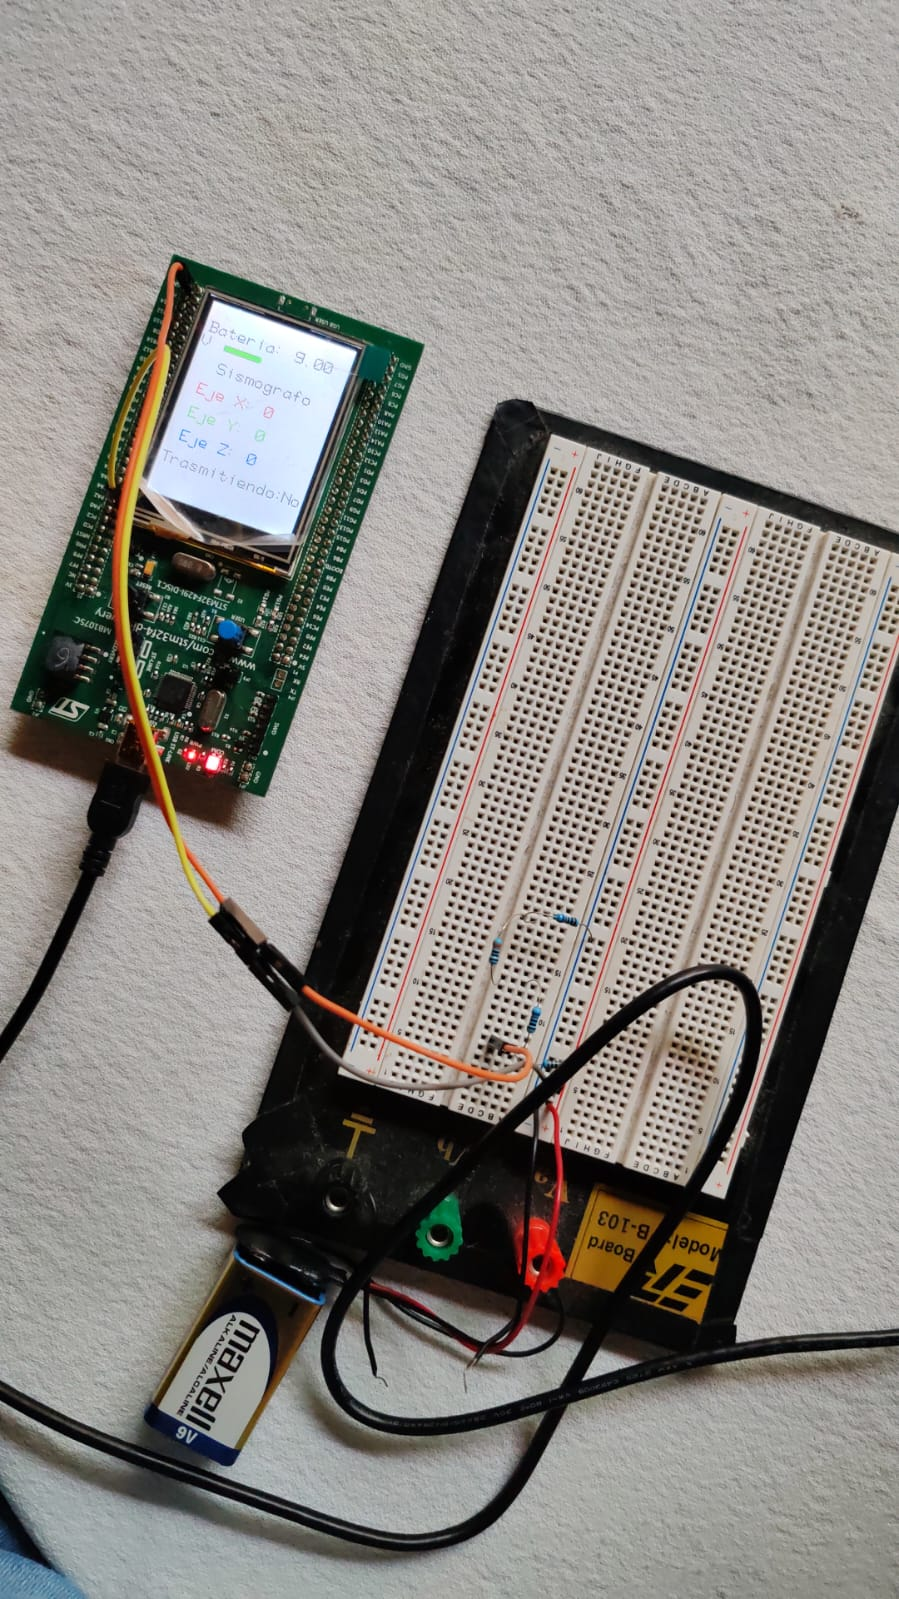
\includegraphics[scale=0.2]{images/lab4.jpeg}
    \caption{Diseño del circuito}
    \label{fig:circuito}
\end{figure}


\newpage


\subsection{Funcionalidad de Hardware}

Para el diseño del circuito implementado se diseñaron los siguientes valores de las resistencias.

\begin{figure}[H]
    \centering
    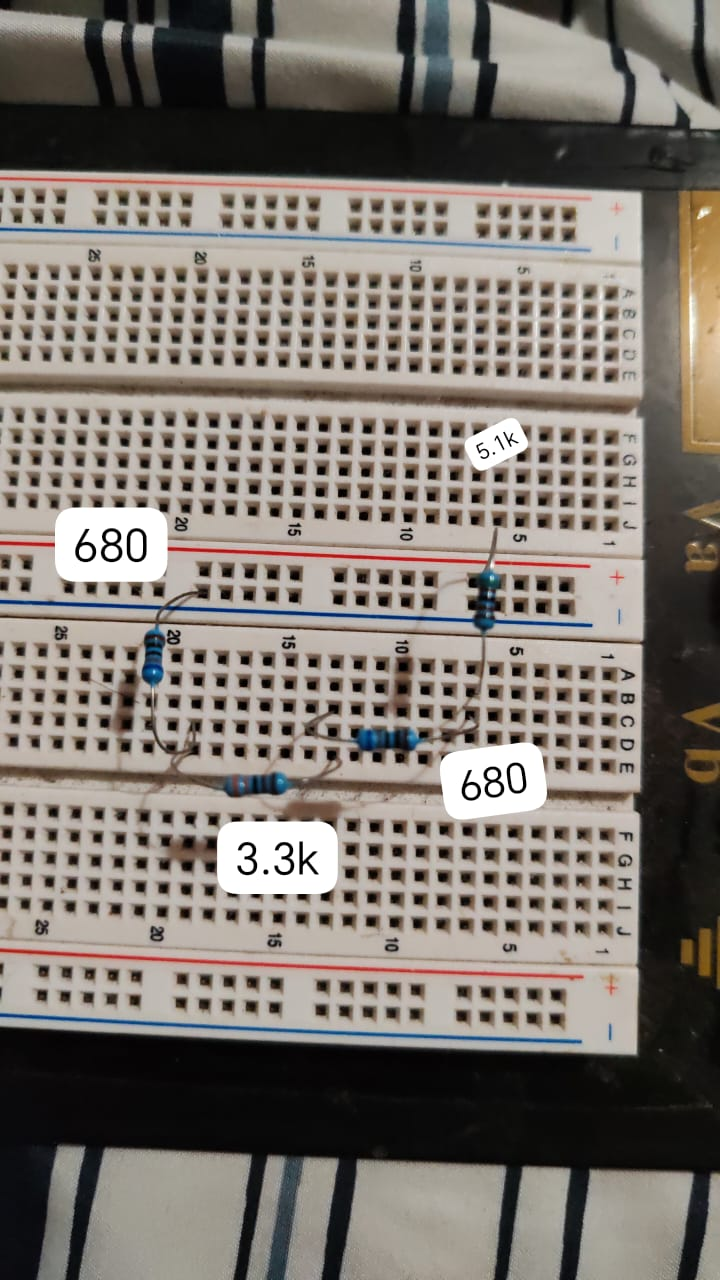
\includegraphics[scale=0.2]{images/Resistencias.jpeg}
    \caption{Diseño del circuito}
    \label{fig:circuito}
\end{figure}

En la figura previamente presentada, se observa la implementación de varios componentes. Específicamente, se han utilizado dos resistencias de 680 $\Omega$, una resistencia de $3.3 K\Omega$ y otra resistencia de $5.1 K\Omega$.

Estos valores de las resistencias y su configuración consisten en una división de tensión con el fin de reducir la tensión de entrada de 9V proveniente de la batería externa a un nivel seguro para el microcontrolador que en este caso puede soportar que es hasta 5 V. 

Por lo tanto aplicando la ecuación para una división de tensión se obtiene que:

\begin{equation}
    V_{out} = V_{in} * (\frac{R2}{R1 + R2})
\end{equation}


\begin{equation}
    V_{out} = 9V * (\frac{5.1k\Omega}{3.3k\Omega + 2 \cdot 680 \Omega + 5.1k \Omega})
\end{equation}

\begin{equation}
    V_{out} = 4.7 V
\end{equation}

Es importante notar que se hizo este arreglo de resistencias, porque luego de varias pruebas de prueba y error, con estos valores se obtuvo un valor de tensión funcional para el microcontrolador. A continuación se aprecia el valor obtenido midiéndolo con el multímetro.

\begin{figure}[H]
    \centering
    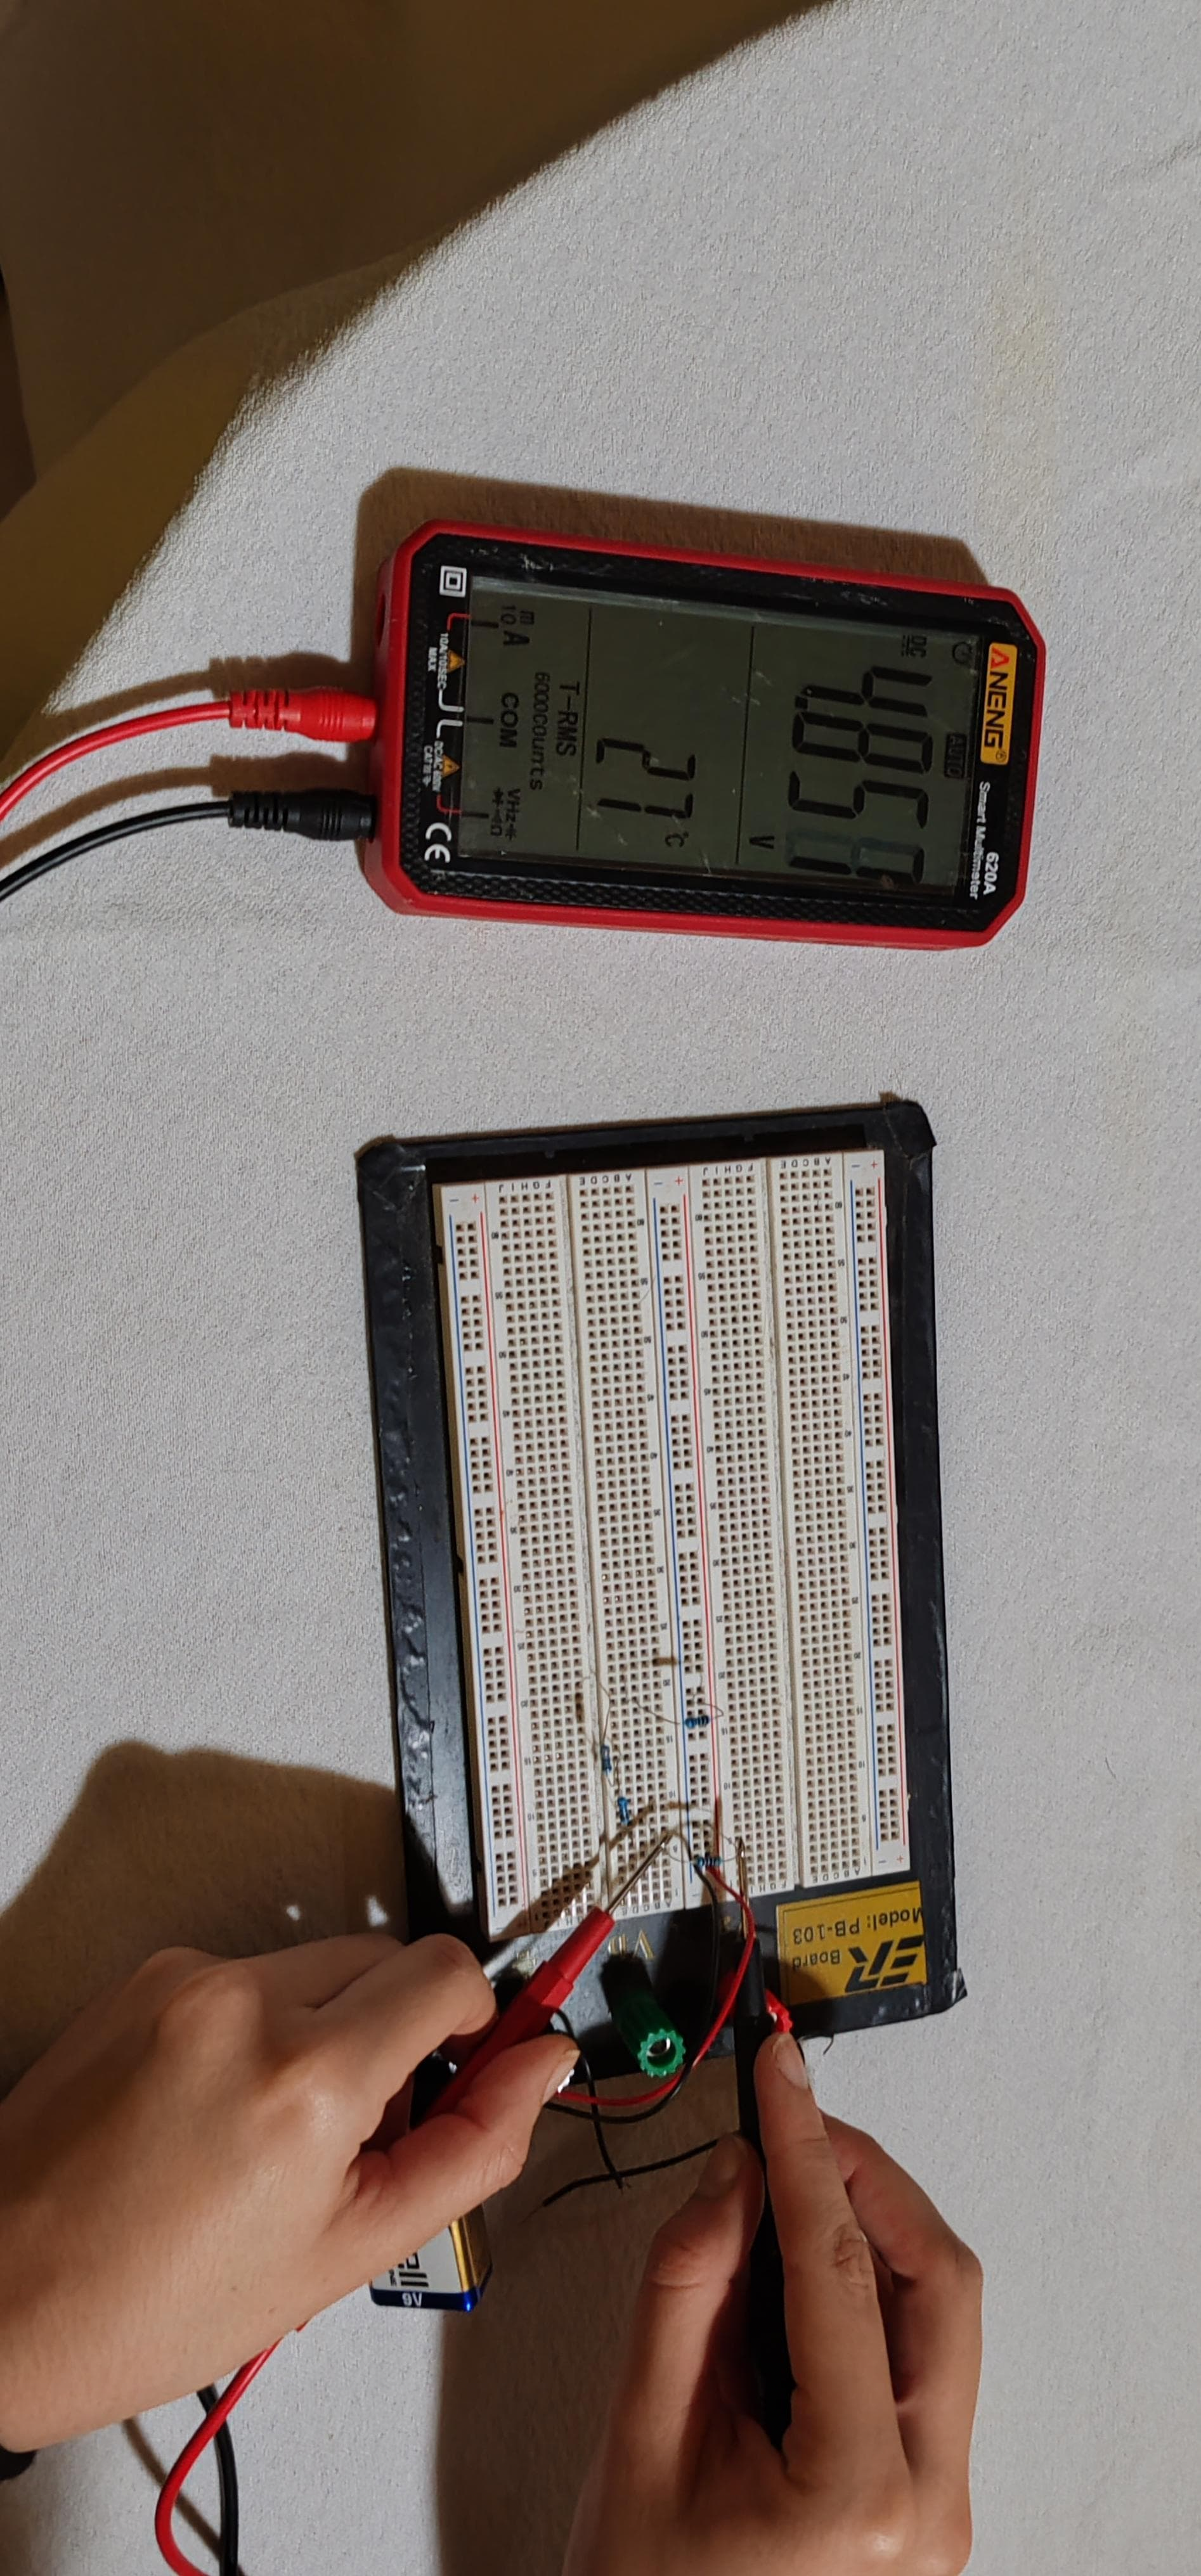
\includegraphics[scale=0.1, angle=90]{images/Medicion.jpg}
    \caption{Medición del valor de tensión luego de la división de tensión}
    \label{fig:circuito}
\end{figure}

Se puede apreciar que se obtuvo un valor de \textbf{4.857 V}, el cuál se encuentra dentro del rango funcional del microcontrolador y muy cercano al calculado teóricamente con la fórmula de división de tensión. 


\subsection*{Funcionamiento de la Pantalla}

\begin{description}
    \item[Nivel de batería] Se representa tanto en formato de texto como gráficamente mediante una barra que cambia de color según la carga.
    \item[Datos del sismógrafo] Los valores de los ejes se muestran con colores distintos: rojo, verde y azul para los ejes X, Y y Z respectivamente.
    \item[Estado de transmisión] Indica si los datos se están transmitiendo o no.
\end{description}
El funcionamiento de la pantalla se puede observar en la siguiente imagen:
\begin{figure}[H]
    \centering
    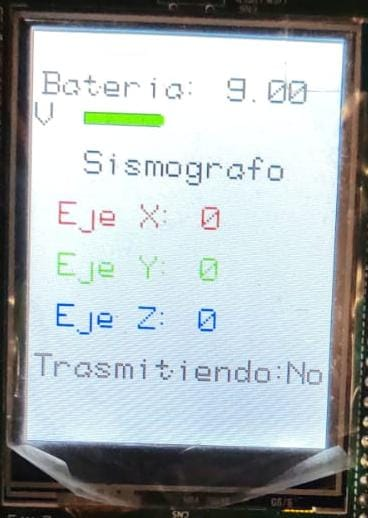
\includegraphics[scale=0.25]{images/pantalla.jpeg}
    \caption{Datos impresos en pantalla.}
    \label{fig:pantalla}
\end{figure}

\subsection*{Interacción con LEDs}

Adicionalmente, el sistema utiliza LEDs para ofrecer retroalimentación sobre ciertos estados, complementando así la información mostrada en la pantalla.

\newpage

\subsection{Funcionalidad de Software}

Para la funcionalidad del Software se implementó un código en el lenguaje de programación C  donde se cubren múltiples funcionalidades relacionadas con la interacción de los periféricos y sensores como un giroscopio basándose en lógica que fue implementada en la librería de ejemplos del microcontrolador STM32: \textit{libopencm3-examples}.

Es importante señalar nuevamente que gran parte de la configuración realizada fue para configurar un giroscopio que es la base del funcionamiento de un sismógrafo, esto debido a que gracias al giroscopio se puede interactuar con la posición del dispositivo en las coordenadas X,Y y Z. Entre las definiciones relacionadas con el giroscopio se encuentran la identificación del dispositivo, registros de control, registros de datos, entre otros. Esto es con el fin de configurar y obtener datos del giroscopio. Se hizo uso de una \textit{struct} en C llamada \textit{gyro} que tiene tres enteros de 16 bits para almacenar los valores de los ejes X, Y y Z del giroscopio.

Es importante notar además que se definen funciones para realizar transacciones SPI con el giroscopio y configurar la interfaz SPI. El SPI es un protocolo de comunicación para que pueda existir la comunicación entre periféricos. Además se implementó otro protocolo de comunicación llamado USART (Universal Synchronous Asynchronous Receiver Transmitter) para la transmisión de datos que genera el giroscopio. En este caso, se utiliza para transmitir datos a través del pin GPIO9 del puerto A con una velocidad de transmisión de 115200 bps.

La pantalla requiere un proceso de inicialización y configuración. Este proceso incluye la activación de ciertos periféricos, configuración de pines y comunicación inicial con la pantalla para establecer parámetros operativos.

El sistema utiliza una biblioteca gráfica que ofrece funciones para diferentes operaciones gráficas como:
\begin{itemize}
    \item Limpiar la pantalla.
    \item Configurar el tamaño y color del texto.
    \item Dibujar y rellenar rectángulos.
\end{itemize}
Para la configuración de los pines, se conectó de la siguiente manera:

\textbf{GPIOC, GPIO1:} \\
Utilizado para controlar el Chip Select (CS) del giroscopio durante las transacciones SPI. 

\textbf{GPIOF, GPIO7 | GPIO8 | GPIO9:} \\
Estos pines se configuran para el modo de función alternativa (AF), específicamente para la interfaz SPI con el giroscopio. La función exacta de cada uno no se detalla, pero generalmente en SPI estos pines corresponden a MISO (Master In, Slave Out), MOSI (Master Out, Slave In) y SCLK (Serial Clock).

\textbf{GPIOA, GPIO9:} \\
Configurado para transmitir datos desde USART1. Por este medio es donde se transmiten los datos y son interpretados por un script de \textit{Python}.

\textbf{GPIOA, GPIO0:} \\
Se configuran como entradas. 

\textbf{GPIOG, GPIO13 y GPIO14:} \\
Se configuran como salidas. 

\textbf{GPIOA, GPIO3:} \\
Utilizado para leer el nivel de batería mediante el ADC. Es una entrada analógica que recoge los valores de voltaje de la batería.

A continuación se muestra un diagrama de bloques del funcionamiento básico del sismógrafo

\begin{figure}[H]
    \centering
    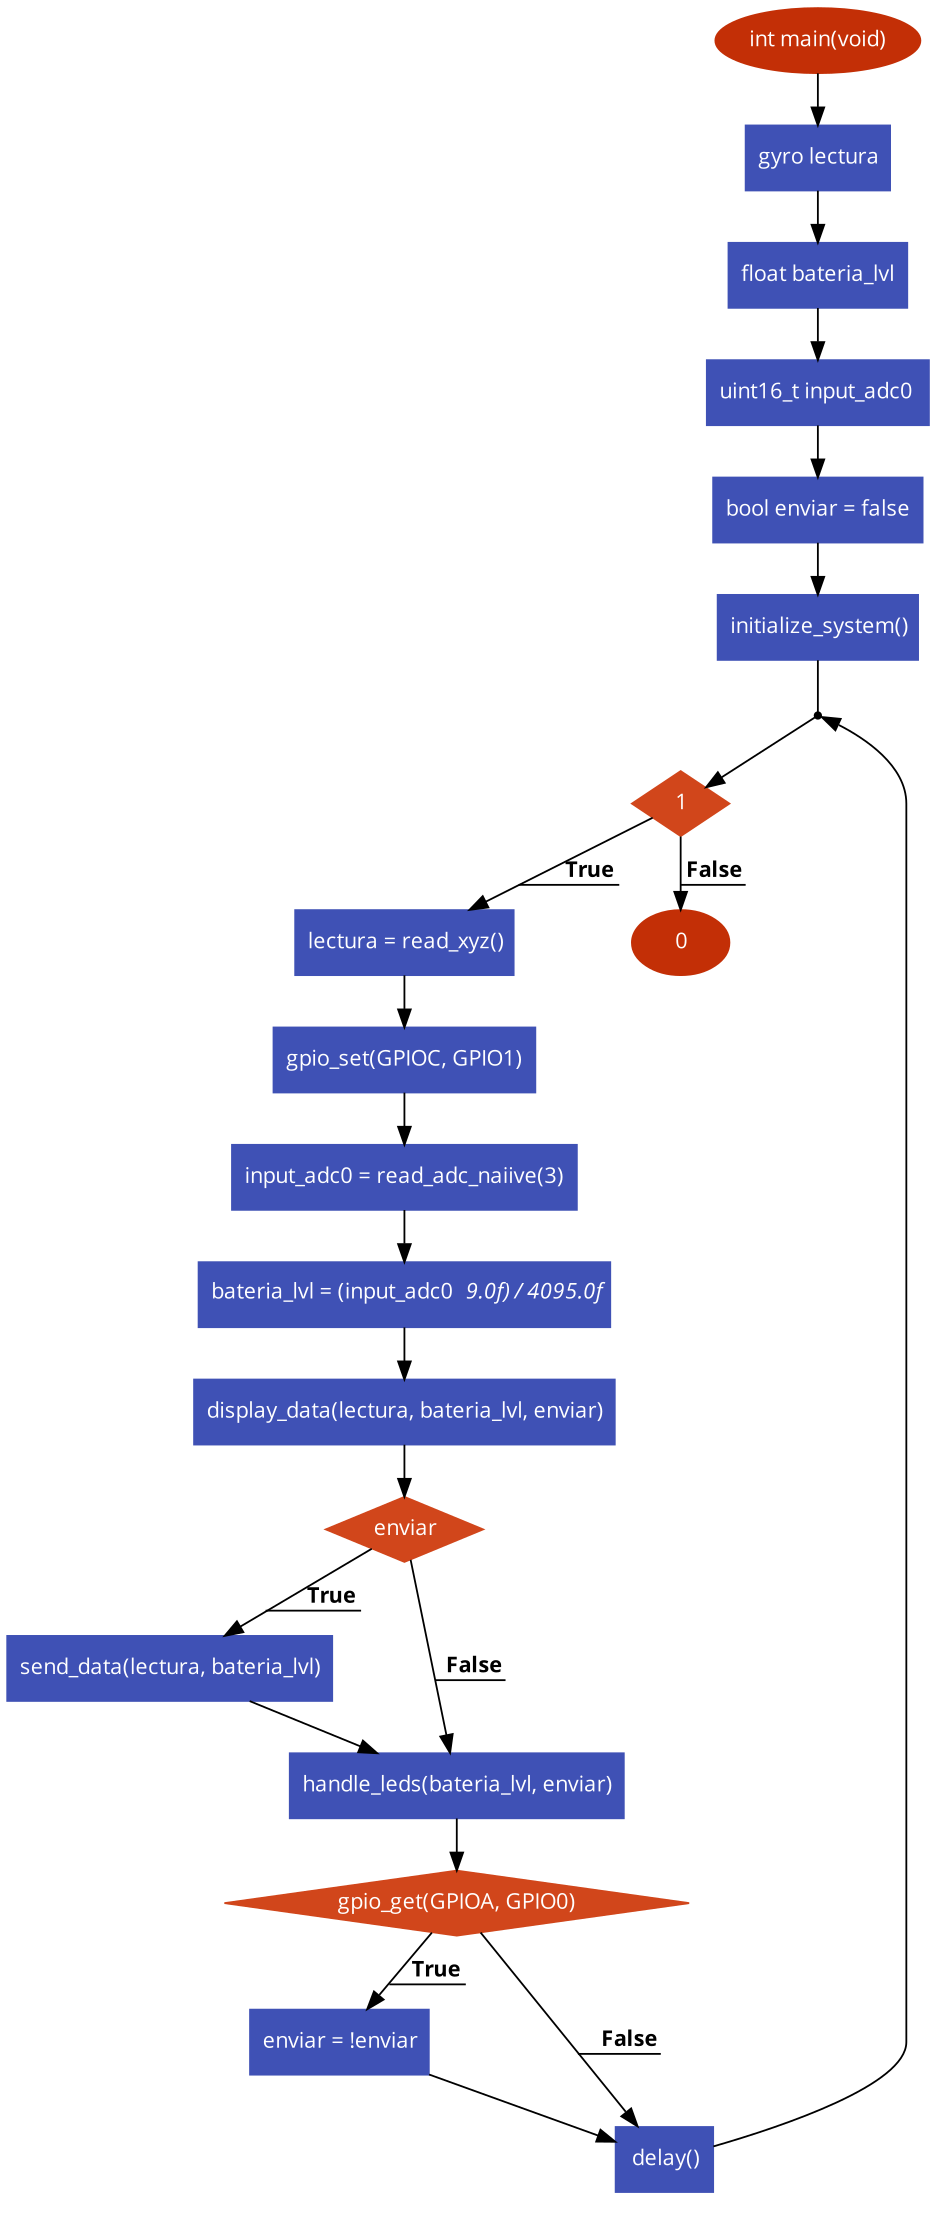
\includegraphics[scale=0.25]{images/Bloques.png}
    \caption{Diagrama de bloques del código implementado}
    \label{fig:circuito}
\end{figure}

\newpage

\textbf{\title{Código en Python}}

Además es importante destacar que también se implementó otro código en el lenguaje de programación \textit{Python}. Este otro código, tiene la finalidad de leer/escribir el puerto USB y que pueda enviar la información del giroscopio y nivel de batería para ser desplegados en un dashboard de la plataforma Iot thingsboard. 

El código se estructura en una clase principal denominada \textit{IOTClient}, la cual encapsula todas las funciones necesarias para establecer las conexiones, leer los datos del sensor y enviarlos al servidor. Hay 3 elementos importantes en el código para su funcionamiento:

\begin{itemize}
    \item time: maneja las pausas entre envíos de datos
    \item json: convierte los datos a formato JSON
    \item serial: permite la comunicación a través del puerto serial
    \item paho.mqtt.client: logra la interacción con el protocolo MQTT.
\end{itemize}

La clase IOTClient mencionada anteriormente, maneja la configuración de las conexiones, la lectura de datos del sensor, y su envío al servidor. Al iniciar, establece las conexiones serial y MQTT, e inicia un bucle que lee los datos del sensor, los convierte a formato JSON, y los publica en el servidor MQTT con una pausa entre envíos. Si se ejecuta el script directamente, se crea una instancia de IOTClient y se inicia este proceso, permitiendo la transmisión continua de datos del sensor al servidor MQTT.

\textbf{\title{Iot Thingsboard}}

Luego del correcto funcionamiento del sismógrafo y la implementación del código en Python para leer/escribir el puerto USB, se configuró la plataforma de Iot Thingsboard para poder manejar y visualizar los datos enviados y recibidos. Para la configuración en la plataforma, se utilizó la cuenta que fue creada por el profesor con el correo institucional. 

A continuación se puede apreciar la data visualizada del sismógrafo mediante dicha plataforma:

\begin{figure}[H]
    \centering
    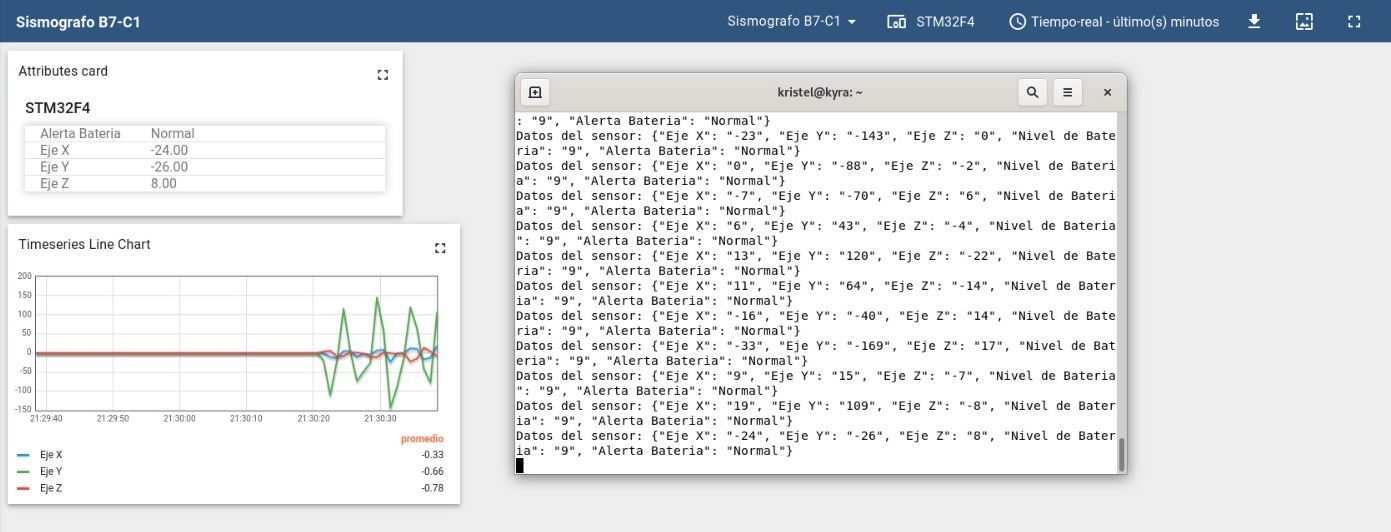
\includegraphics[scale=0.32]{images/thingsboard.jpeg}
    \caption{Sismógrafo en plataforma ThingsBoard}
    \label{fig:thingsboard}
\end{figure}


